\documentclass[10pt,a4paper]{article}
\usepackage[utf8]{inputenc}
\usepackage{amsmath}
\usepackage{amsfonts}
\usepackage{amssymb}
\usepackage{german}
\usepackage{fancyhdr}
\usepackage{graphicx}
\usepackage{geometry}
\usepackage{color}
\usepackage[usenames,dvipsnames,table]{xcolor}
\usepackage{DejaVuSans}
\usepackage[T1]{fontenc}

\usepackage{cite}
\usepackage{float}
\usepackage{wrapfig}
\usepackage{lscape}
\usepackage{rotating}
\usepackage[nottoc]{tocbibind}
\usepackage{epstopdf}
\usepackage{graphicx}
\usepackage{tabularx}
%\usepackage{floatrow}
\usepackage[T1]{fontenc}
\usepackage[utf8]{inputenc}
\usepackage{mathptmx}
\renewcommand{\rmdefault}{ptm}

\renewcommand*{\familydefault}{\sfdefault}
\geometry{verbose,a4paper,tmargin=35mm,bmargin=35mm,lmargin=25mm,rmargin=25mm}
\author{Dominik Heeb, Fabian Keller}
\title{Projektplan Bachelorarbeit}
\pagestyle{fancy}
\fancyhead{}
\fancyhead[L]{Projektplan - Verkehrsmodell-Fallstudien-Editor}
\fancyhead[R]{Domink Heeb, Fabian Keller}
\fancyfoot{}
\fancyfoot[R]{Seite \thepage}
\begin{document}
\begin{titlepage}
	\begin{Huge}
		\begin{center}
				Projektplan \\Verkehrsmodell-Fallstudien-Editor\\[2.0cm]
		\end{center}
	\end{Huge}
	
	\begin{center}
		\begin{Large}
				von Dominik Heeb, Fabian Keller\\[1.0cm]
		\end{Large}
		\begin{large}
				Betreuer: Prof. Dr. Luc Bläser
		\end{large}
	\end{center}
\end{titlepage}

\newpage
\tableofcontents 
\newpage

\section{Management Abläufe}
\begin{flushleft}
	Diese Bachelorarbeit wird im Rahmen des Bachelor Studiums an der HSR durchgeführt welches bei erfolgreichem Abschluss mit 12 ECTS Punkten gewertet wird. Ein ECTS Punkt entspricht einem ungefähren Zeitaufwand von 25 bis 30 Stunden. Somit wird von jedem Teammitglied ein Zeitaufwand von ca. 300 bis 360 Stunden erwartet.
\end{flushleft}

\subsection{Zeitliche Planung}
	\begin{flushleft}
Der zeitliche Projektplan zeigt eine grobe zeitliche Übersicht über die gesamte Bachelorarbeit mit den einzelnen Iterationen und Meilensteinen.
	\end{flushleft}
	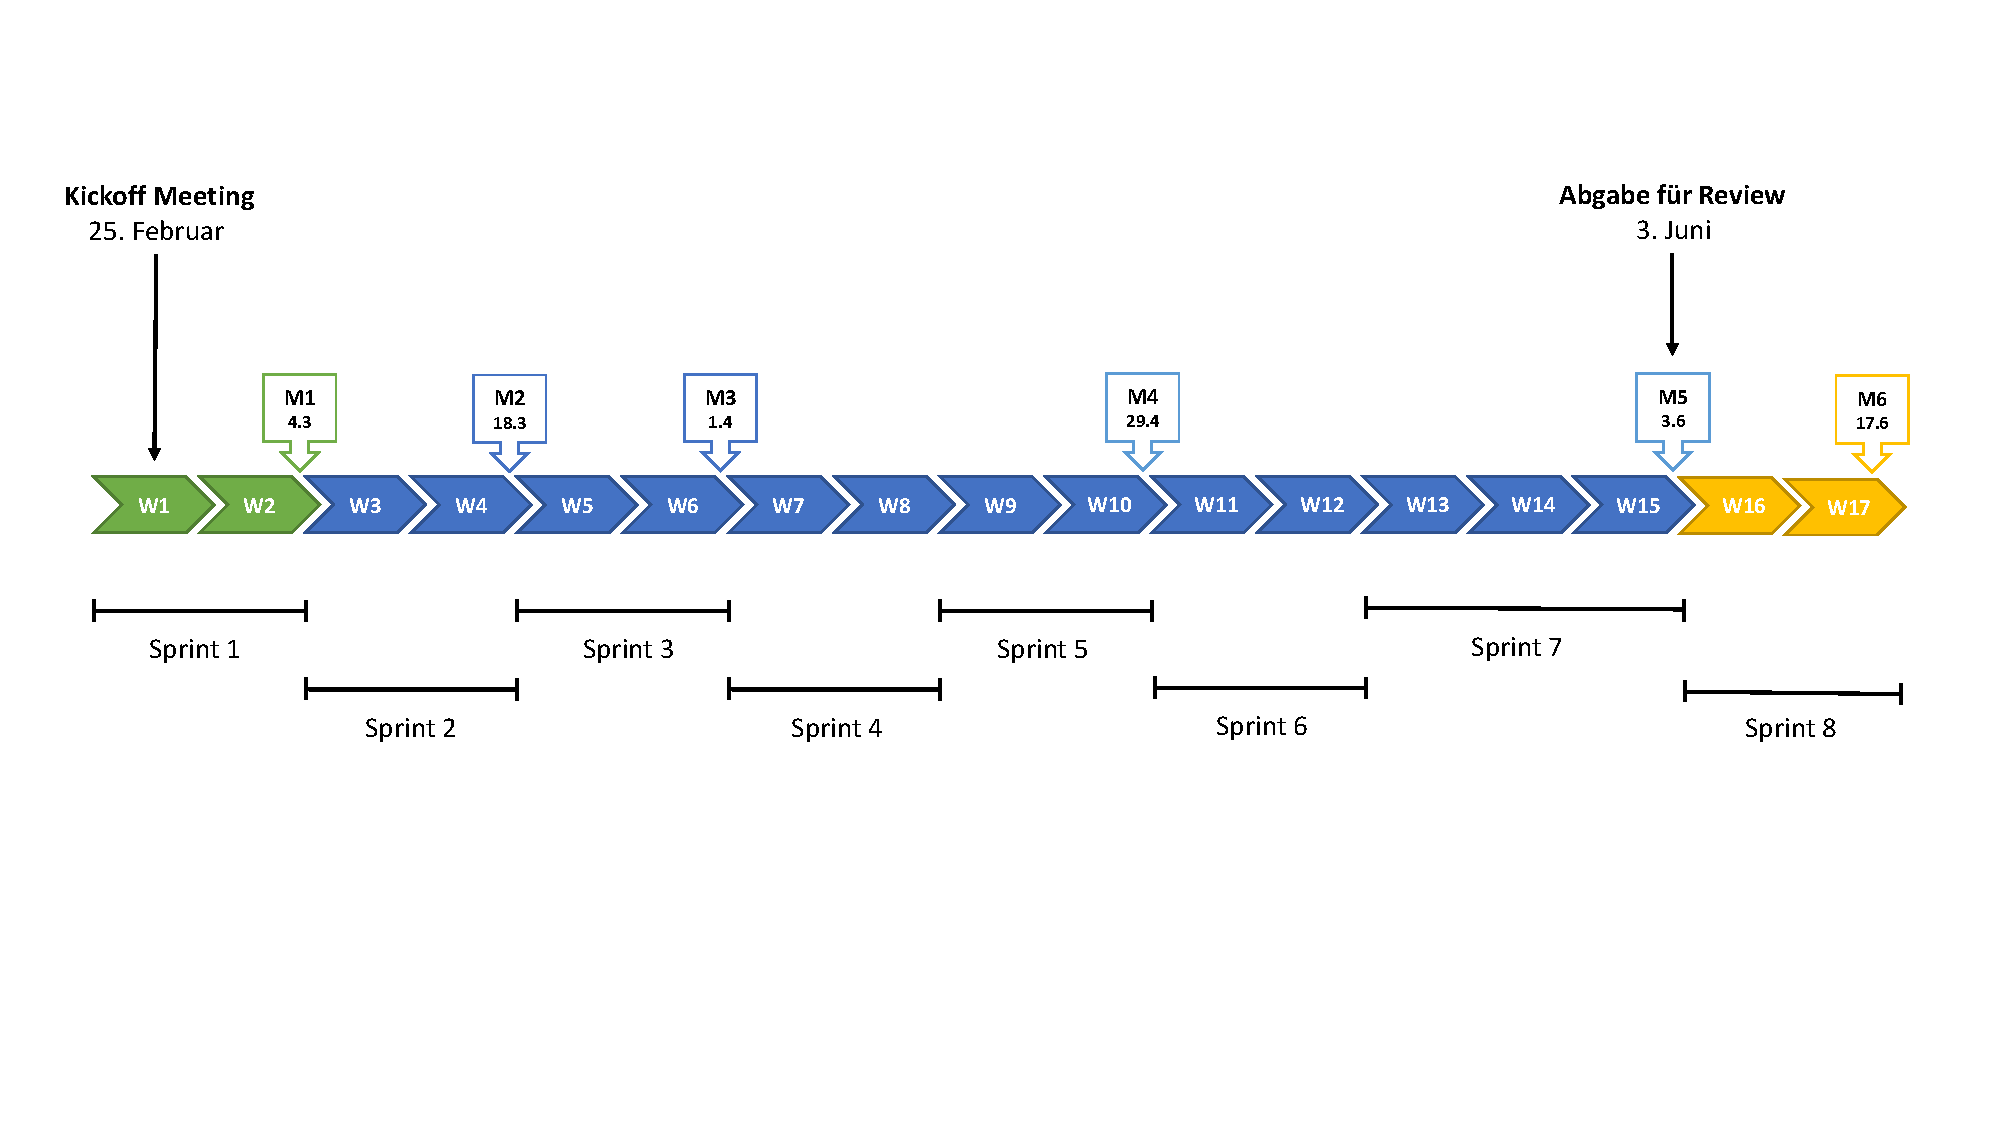
\includegraphics[width=17cm,height=7cm,trim=10mm 40mm 0mm 20mm, clip]{pictures/Meilensteinplan.pdf}

\subsection{Meilensteine}
\begin{flushleft}
Die einzelnen Meilensteine beinhalten folgende Ziele:
\end{flushleft}
\begin{tabular}{cl}
	\textcolor{Orange}{\textbf{M1:}} & Projektplan erstellt, Infrastruktur fertig aufgebaut \\[0.2cm]
	\textcolor{Orange}{\textbf{M2:}} & Prototyp v0.1: Anzeigen von Strassennetz in Online Map Editor \\[0.2cm]
	\textcolor{Orange}{\textbf{M3:}} & Prototyp v0.2: Anzeigen von Parameter zu Strassen in Online Map Editor \\[0.2cm]
	\textcolor{NavyBlue}{\textbf{M4:}} & komplette Verkehrsdaten (Strassennetz, ÖV-Verkehsnetz, Parameter usw.) in Online Map-Editor darstellen\\[0.2cm]
	\textcolor{NavyBlue}{\textbf{M5:}} & Definierte Änderungen können an Verkehrsdaten in Online Map-Editor vorgenommen werden\\[0.2cm]
	\textcolor{Dandelion}{\textbf{M6:}} & Präsentation der Bachelorarbeit, Abgabe Bericht\\
\end{tabular}
\subsection{Besprechungen}
\begin{flushleft}
	Die Besprechung findet jede Woche am Donnerstag im Raum 1.167 um 14:00 Uhr statt. In dieser Besprechung wird der aktuelle Status der Bachelorarbeit und das weitere Vorgehen besprochen und offene Fragen geklärt.\\
Das Projektteam erstellt vor jeder Besprechung eine Traktandenliste und führt ein Sitzungsprotokoll. Dieses Protokoll wird anschliessend an den Betreuer und den Auftraggeber gesendet.
\end{flushleft}
\subsection{Risiken}
\begin{flushleft}
\begin{tabular}{l l l}
Risiko & Wahrscheinlichkeit & Potential\\
\hline
Datenmenge zu gross & mittel & mittel\\
Backend Implementierung zu aufwändig & klein & mittel\\
\end{tabular}\\[0.2cm]
\subsubsection*{Datenmenge zu gross}
Dieses Risiko enthält die Gefahr das durch zu grosse Datenmengen die Client-Side Implementierung des Editor zu aufwändig wird. Die Folge daraus wäre das der Editor nicht zufriedenstellend entwickelt werden kann. Eine Massnahme um die Wahrscheinlichkeit des Eintretens klein zu halten ist es, von Anfang an die Menge der Daten in die Implementierung und Konzeptionierung einfliessen zu lassen.\\[0.2cm]
\subsubsection*{Backend Implementierung zu aufwändig}
Die Konzeptionierung des Verkehrsmodell-Editor behandelt hauptsächlich die Frontend Entwicklung. Wenn der Backend zu komplex wird, bleibt zu wenig Zeit den Frontend ansprechend zu entwickeln. Die Massnahme ist, den Backend auf das Wesentliche zu beschränken und die Entwicklung des Frontend in den Vordergrund zu stellen. Funktionen für den Backend sollten wenn sie zu viel Zeit brauchen vereinfacht werden.\\

\end{flushleft}

\definecolor{lightgray}{rgb}{0.83, 0.83, 0.83}
%Since the PHA worksheet is wide, start in a new page by using begin {landscape} command.
\begin{landscape}
\begin{table}[H]
\scriptsize
\caption{Risikoanalyse (fortlaufend)}
\begin{tabular}{p{0.5cm}p{4cm} p{1.5cm} p{1.5cm} p{1cm} p{2cm}p{1.5cm}p{1cm}p{2cm}p{1.5cm}}
\hline & & & & \bf Initiales Risiko \cellcolor{lightgray} & \cellcolor{lightgray} & \cellcolor{lightgray} & \bf Aktuelles Risiko & & \\ [13pt]
\bf \bf ID & \bf Risikobezeichnung & \bf Risikoklasse & \bf Mögliche Risikoursache & \ \bf EW \% \cellcolor{lightgray} & \bf Schadenshöhe (h) \cellcolor{lightgray} & \bf Risikowert (h) \cellcolor{lightgray} & \bf EW \% & \bf Schadenshöhe (h) & \bf Risikowert (h) \\
\hline
&&&&&&&&&\\
1 & Datenmenge zu gross & mittel \cellcolor{yellow!50} &&&&&&&\\
%Example- & 5g & & Early launch of life crafts & Improper evacuation procedure & 3 & 4 & \cellcolor{red!50} 12 & Plans for Emergency Preparedness based on facility design & 2& 2& \cellcolor{green!50} 4 \\ %cell color can be changed to red or yellow- {yellow!50} or red -{red!50}

%add more rows as required

\hline
\end{tabular}
\end{table}
\end{landscape}
\newpage
\section{Vorgehen}
\subsection{Projektmanagement}
\subsubsection{Aufbau}
\begin{itemize}
	\item Elaboration: 
	\item Construction: 
	\item Transition: 
\end{itemize}
\subsubsection{Tools}
Für das Projektmanagement werden folgende Tools verwendet:
\begin{itemize}
\item JIRA: für die Planung und Verwaltung der Arbeitspakete.
\item GitHub: Der Code und die Dokumentation werden über Github Repositories verwaltet
\item CI Server (JetBrains TeamCity): Mittels eines CI Server wird die Qualität und Lauffähigkeit des Codes geprüft
\item TexMaker: Latex Editor für die Dokumentation
\item IntelliJ IDEA 15: IDE für Java Entwicklung
\end{itemize}
\subsection{Entwicklung}
\subsubsection{Vorgehen}
Die Entwicklung der Bachelorarbeit wird als Agiles Softwareprojekt aufgebaut.
\subsubsection{Unit Testing}
\subsubsection{Code Reviews}
Code Reviews und Pair Programming sind Methoden um die Qualität des Codes innerhalb des Teams hoch zu halten
\subsubsection{Code Analyse}
\subsubsection{Code Style Guidelines}
\end{document}